~
\newpage
\section{Carbon Pricing \& Air Pollution Disparities in California}

\subsection{Empirical Strategy}

The goal of this chapter is to take the model of electricity generation and environmental inequality presented in Chapter 4 and apply it to simulate the effects of California's emissions trading scheme within the western US power grid, the Western Interconnection. The proceeding sections will discuss the data the simulation uses and the results of the simulation. First though, this section will outline the approach I use to operationalize the model in Chapter 4. 

As discussed in Chapter 3, the Western Interconnection is the power grid that connects much of the western half of the contiguous US. Figure \ref{wecc_regions} displays this region. The power grid is further split into four subregions: the California-Mexico Power Area (CAMX), the Northwest Power Pool Area (NWPP), the Rocky Mountain Power Area (RMPA), and the Arizona-New Mexico-Southern Nevada Power Area (AZNM). However, the US Energy Information Administration does not report the necessary data for the NWPP and RMPA separately, so this analysis divides the Western Interconnection into three regions: California, the Northwest, and the Southwest. 
\begin{figure}
    \centering
    \caption{Western Interconnection Subregions \label{wecc_regions}}
    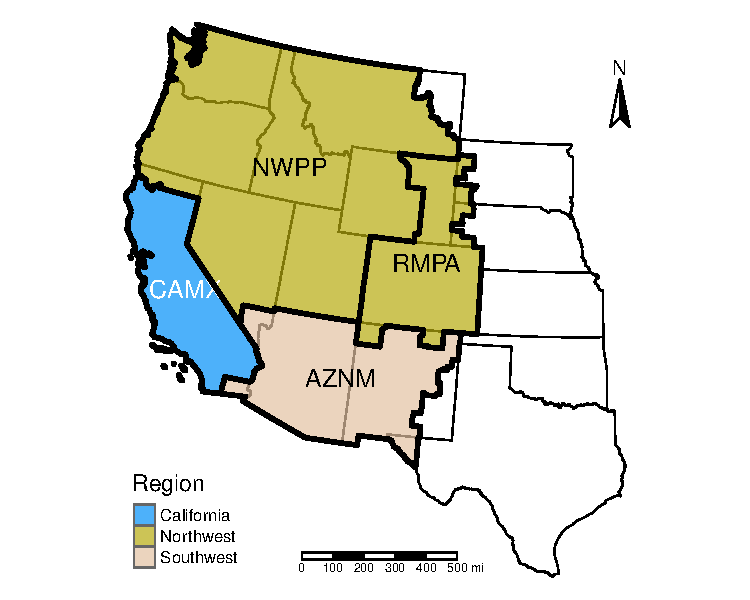
\includegraphics[width=0.8\textwidth]{figures/chapter3_figures/WECC_map.pdf}
    \fignote[1]{Figure displays the subregions of the Western Interconnection. These subregions are a unit of geography set by the North American Electric Reliability Council (NERC). NERC determines these regions based off of the connections/boundaries between balancing authorities, the administrative unit of the US power grid. These regions are the California-Mexico Power Area (CAMX), the Northwest Power Pool Area (NWPP), the Rocky Mountain Power Area (RMPA), and the Arizona-New Mexico-Southern Nevada Power Area (AZNM). The EPA reports data for each of the four NERC regions, but the EIA only provides electricity demand data for the NWPP and RMPA together. These two subregions are treated as one throughout the paper, and future chapters will model just the three regional markets displayed: the California market, the Southwest market, and the Northwest market. Shapefiles for the regions come from \cite{HIFLD_nerc}.
    }
\end{figure}

The central goal of this text is to analyze the effect of carbon pricing on environmental inequality, as measured by the environmental inequality gap (EI Gap) described in Chapter 4. To do so, the simulation model considers a set of policy scenarios with a range of carbon prices and measures the resulting disparities in air pollution under each policy scenario. Table \ref{policy_scenarios} outlines these different policy scenarios. For policy scenarios where all else is equal except the carbon price, the causal effect of the incremental change in the carbon price on the EI Gap is given by the difference in the EI Gap between the two scenarios. 

Other than the carbon price itself, another relevant concern in the model is the presence of Border Carbon Adjustments (BCAs). Recall from section 2.5 that BCAs impose charges on imports or possibly rebates on exports of emissions intensive goods with the intention of preventing emissions leakage. The potential for carbon pricing to redistribute economic activity and the associated environmental consequences across jurisdictions is the primary motivation for creating a multi-region model of electricity generation in Chapter 4. Given the importance of these inter-regional dynamics in the model, the policy scenarios also vary in their use of BCAs. In the first five policy scenarios, there is no BCA; California power plants face a carbon price, but generation outside of California that is sold in California does not face a carbon price. In the final four policy scenarios, there is a uniform BCA. Under a uniform BCA, all of California's electricity imports face a uniform carbon price. The charge on electricity imports (\$/MWh) is the product of the domestic price of emissions (\$/tonne CO$_2$e) and the average emissions intensity of electricity (tonnes CO$_2$e/MWh) generated in the Western Interconnection outside of California.\footnote{I recover the average emissions intensity of power generated in the Western Interconnection outside of California from the 2019 eGRID dataset.} Together, the nine policy scenarios enable the simulation to speak to the effect of carbon pricing on generation, greenhouse gas emissions, local air pollutant emissions, and disparities in local air pollutant emissions.

\begin{table}
    \centering
    \caption{Summary of Policy Scenarios \label{policy_scenarios}}
    \begin{tabular}{c c c}
        \hline\hline
        Policy Scenario & BCA? & Carbon Price (\$/tonne)\\
        \hline
        A & No & 0\\
        B & No & 20\\
        C & No & 40\\
        D & No & 60\\
        E & No & 80\\
        F & Yes & 20 \\
        G & Yes & 40 \\
        H & Yes & 60 \\
        I & Yes & 80 \\
    \hline    
    \end{tabular}
    \fignote[1]{Table summarizes the policy scenarios simulated. The Border Carbon Adjustment (BCA) in each scenario that uses a BCA is a uniform BCA, meaning that all electricity imports face a uniform carbon price. This carbon price is the average emissions intensity of all electricity generation in the exporting region times the domestic carbon price. In the actual implementation of the simulation model, there is an additional scenario that considers the situation where there would be a BCA but the carbon price is zero. This sceanrio is equivalent policy sceanrio A and is just used to help ensure the model functions properly. Each policy scenario is also re-considered under higher investment cost, a point addressed later in the section.
    }
\end{table}

With the policy scenarios established and provided all other necessary data is available, the simulation must just run the series of constrained optimizations laid out in the previous chapter. However, the size of this problem is prohibitive. There are 481 qualifying power plants in the Western Interconnection, each with four discrete choices (operate for California, operate of the Northwest, operate for the Southwest, and do not operate), meaning that solving the generation problem for a single hour with a given investment scenario would involve finding the least cost generation profile out of $4^{481}$ distinct generation profiles. This problem of course grows even larger when a large number of investment profiles and hourly demand schedules are under consideration. 

Following the standard approach in the literature for dealing with these prohibitively large optimization problems, I use $k$-means clustering to simplify the problem by forming representative power plants and a representative demand schedule. 

As in \cite{fowlie2021border}, I use $k$-means clustering to group the hourly demand schedule into twenty-four clusters. This takes the three years of hourly electricity demand data from each region and parses it into a representative day. In some analyses, like analyzes concerned with a dynamic problem or performance under extreme situations, simplifying the demand schedule into a single day would not be desirable. In this case though, the analysis is primarily concerned with average outcomes that unfold over the course of a few years, so this strategy greatly reduces the computational burden of the model without any meaningful detriment to the interpretation of the results. 

Similarly, I use $k$-means clustering to cluster power plants into generating groups. Because power plants from different regions will differ in the carbon price they face, power plants in each group must all be located in the same region. Similarly, because power plants with different fuels will differ in the fuel prices they face, power plants in each group must all use the same fuel. With these two boundaries set, I perform $k$-means clustering on all power plants in a region based on their nameplate capacity and their heat rate. In each region, I create one group for coal power plants, eight groups for gas power plants, and one group for oil power plants. Together, there are thirty power plant groups, ten for each of the three regions. For each of these groups, I create a single representative power plant, endowed with the total nameplate capacity and the average heat rate of all power plants in the group. 

The generation optimization problem with these thirty representative power plants is identical to the optimization in equation \ref{C_star}, with the one modification that in their implementation, representative power plants have a continuous choice set. Let $q_{gtr}$ be the total generation of the power plants in group $g$ at time $t$ for region $r$. Although $q_{itr}$ is discrete in Chapter 4, here $q_{gtr}$ is a continuous variable greater than zero, such that
\begin{equation}
    \sum_{r = 1}^3 q_{gtr} \leq 0.9 \cdot \overline{q_{gtr}},
\end{equation} 
where $\overline{q_{gtr}}$ is the sum of the nameplate capacities of all power plants in group $g$. In practice, almost no power plants have a capacity factor greater than 0.9, meaning that even the lowest cost power plants are only able to run 90\% of their potential capacity. The constant $0.9$ in the capacity constraint above reflects this reality that power plants cannot run at full capacity all the time, but must occasionally stop operating or operate at less than their maximum rated capacity. 

The results of the generation optimization for a given investment profile and demand schedule contain the total quantity of electricity generated by each of the thirty representative power plants for each of the three regions. Ultimately though, the model must predict generation and emissions for individual power plants. To compute the generation of individual power plants from the generation of the representative power plant groups, I start by summing the generation of each power plant group across the three regions to find the total generation of the power plants in the group during the given period. Using the total nameplate capacity of power plants in the group, I calculate the capacity factor (actual generation/maximum possible generation) of each representative power plant, and then assign this capacity factor to each power plant in that group. For instance, suppose power plant $i$ has a nameplate capacity of 100 MW and is in group $g$. If the total nameplate capacity of group $g$ is 1000 MW and the simulated generation of group $g$ in the period is 500 MW, then the capacity factor of group $g$ is 0.5. Then I compute the generation of power plant $i$ as the product of the group $g$'s capacity factor and $i$'s nameplate capacity, 50 MW. This means that all power plants in the same generation group end up with an identical distribution of capacity factors, but still vary by their total generation in proportion to their nameplate capacity. 

To implement the investment optimization, I follow largely from \cite{weber2021dynamic}, and start by restricting the number of investment options of power plants to a binary choice. Each power plant can either make an investment to lower its heat rate by 1.5\% or not invest at all. Thirty power plant groups is an acceptable number for the generation optimization, but because simulating a single investment scenario involves working through many generation optimizations, thirty representative power plants is too large for the investment optimization. To simplify this, I perform $k$-means clustering on the generation groups themselves, this time based only the average heat rate of the group, creating two clusters in California and two clusters outside of California.\footnote{Oil power plants are excluded from the investment decision and are assumed to make heat rate improvements. These plants have unusually high heat rates and expensive fuels that would motivate investment. They make up a small share of all available generation, so this assumption does not have strong implications.} With four clusters that each make a binary choice, there are $2^4 = 16$ investment scenarios. Each investment scenario identifies which of the thirty representative groups of power plants invests in a heat rate improvement that will reduce the generation group's average heat rate by 1.5\%. The optimization program loops through each of these sixteen investment scenarios and then reports the results of the investment scenario that had the least cost over the three year period. 

The investment cost function comes from \cite{weber2021dynamic}. Typically, the parameters of the investment cost function would need to be fit using a maximum likelihood estimation routine, but in this case, \cite{weber2021dynamic} has already estimated the parameters of this cost function. To complete the implementation of the investment decision model, I employ Weber's calibrated investment cost function. The power plants Weber calibrates this investment cost function on are all gas power plants in California, and it possible that these costs do not generalize easily to the wider variety of power plants considered in this analysis. Later results suggest that these costs may be too low, so I also consider how investment decisions change when these investment costs are raised by an order of magnitude in Appendix A.5. 

Having simplified the set of investment decisions, the set of power plants, and the set of demand profiles, I simulate the policy scenarios from Table \ref{policy_scenarios}. I implement the optimization program in Python using scipy.optimize.minimize, and let the initial point for each optimization be a vector of generation that corresponds to the situation where each representative power plant produces just under 90\% of its capacity for domestic demand only. Using the technique previously described, these results for the generation of each group of power plants is used to compute the generation for each individual power plant for each representative hour. Annual generation totals are computed by taking the appropriate weights from each representative hour to form totals for a representative day, and multiplying by 365. Greenhouse gas emissions and local air pollutant emissions for each power plant are calculated by multiplying the generation of each power plant by the emissions intensities of each pollutant for each plant. 

While these power plant-level predictions of generation and emissions are valuable, in it of themselves, they cannot speak to disparities in air pollution concentrations. The model in Chapter 4 builds the EI Gap by first designating communities as either ``Disadvantaged'' or ``Nondisadvantaged,'' a terminology that follows from California's SB 535. This bill requires that a proportion of the revenue raised through the state's emissions trading program go directly to projects in disadvantaged communities. To support this policy, California's EPA has developed a data-based approach to designating Census tracts as disadvantaged. Based on the technique California's EPA uses to determine the status of each Census tract in the state, I implement an analogous technique to determine the status of each Census tract in the Western Interconnection. 

Finally, I compute the EI Gap by summing the total emissions of a given local air pollutant in disadvantaged and nondisadvantaged Census tracts, dividing by their total areas, and then finding the difference between concentrations between disadvantaged and nondisadvantaged Census tracts. This is a suboptimal estimate for the pollution concentration, for the primary reason that air pollutants are not bound by Census tract boundaries. Ideally, this analysis might use a chemical dispersion model that would allow me to compute more detailed flows of emissions across the WECC. These models are again prohibitive and incorporating these is outside of the scope of these papers. The measure of concentrations used to form the EI Gap has its weaknesses, but ultimately the annual emissions of a given air pollutant per square mile provides an easy-to-interpret way these results. 


\subsection{Data}

In this section, I provide an overview of the data sources needed to build the simulation. The primary data in this analysis relate to either (1) power plants, (2) electricity demand, or (3) disadvantaged communities, and the section describes the data that compose each of these areas. All data sources I present in this section appear in Table \ref{data_sources} in Appendix A.5.

\subsubsection*{Power Plants}

Data on individual power plants comes from the 2019 version of the Emissions \& Generation Resource Integrated Database (eGRID), a dataset released by the US Environmental Protection Agency (EPA). This dataset complies records on generator characteristics and generation collected through the US Energy Information Administration (EIA) Form EIA-923 and Form EIA-860 with emissions records collected by the EPA's Clean Air Markets Program. eGRID includes all power plants in the US with a registered nameplate capacity, the maximum rated quantity of power a generator can create, of at least 1 MW.\footnote{For context, residential solar panels usually have a nameplate capacity somewhere between 1000 and 3000 W---meaning that the dataset covers all power plants that are at least 300 to 1000 times larger than residential rooftop solar.} At the generator level, this dataset provides key identifying characteristics of each generator including is primary fuel, its location, its age, its nameplate capacity, and whether or not it is operational. From this dataset of all utility-size generators, I filter out generators such that the final dataset includes only generators that were operational in 2019, are within the Western Interconnection, and use either coal, (natural) gas, or oil as their primary fuel. There are a handful of generators---two gas generators and thirteen oil generators---with negative heat rates that indicate the plant actually used more power in 2019 than it generated. Together these have a relatively small capacity of less than 75MW and their capacity factors (proportion of hours they are on) are near zero, meaning that excluding these generators will not influence the results in any meaningful way as they are almost never used and nearing retirement. After filtering down the set of generators, I then aggregate these data up to the power plant level, and merge in additional data collected at the power plant level, including the heat rate and location of the power plant.

\begin{figure}
    \centering
    \caption{Distribution of Power Plants by Region \& Fuel\label{generators_dist}}
    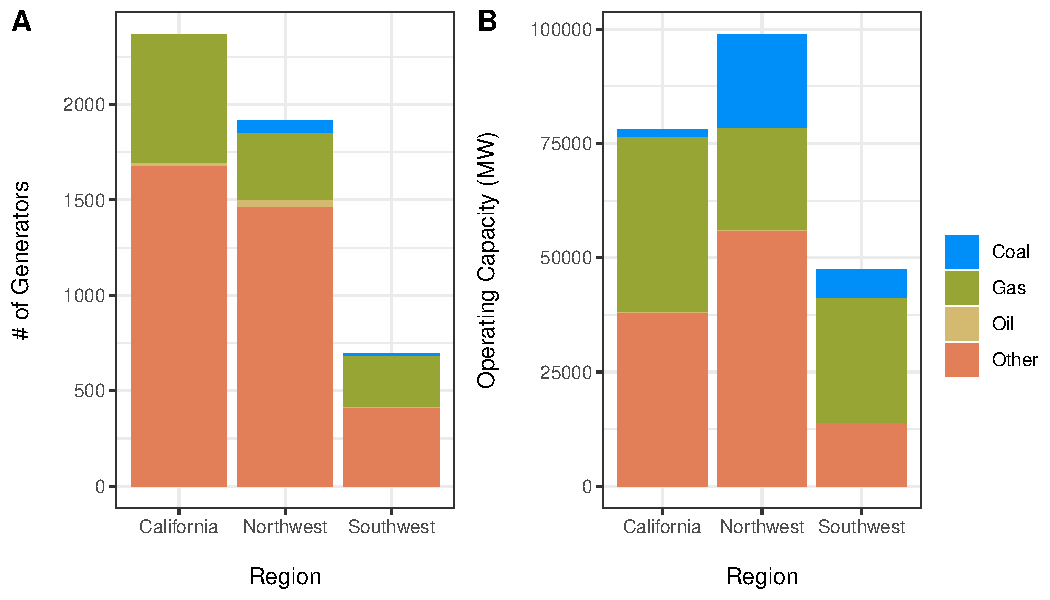
\includegraphics[width=\textwidth]{figures/chapter5_figures/regional_gens.pdf}
    \fignote[1]{
        Panel A breaks down generators by region and fuel type. Generators with fuel type `Other' are not included in the sample, but are displayed for reference on the overall distribution of generation in each region. The bulk of the `Other' fuels category is made up by renewable and nuclear generators. Power plants vary substantially in their nameplate capacities, meaning that Panel A is not an accurate representation of the distribution of available capacity. By comparison, Panel B visualizes the distribution of generating capacity by region and fuel type. The relative size of the bars indicates that coal and natural gas generators have larger nameplate capacities than generators in the `Other' category. 
    }
\end{figure}

Figure \ref{generators_dist} displays the breakdown of generation across the three regions of the Western Interconnection, California, the Northwest, and the Southwest. Panel A looks at all generators across the regions, including those other than the coal, gas, and oil generators that this paper focuses on, for the purpose of comparison. Generators in this ``Other'' category (e.g., renewables and nuclear) account for the majority of generators in each region, and gas plants make up most of the remainder. California has more generators than either of the two regions and almost has as many generators as the two other regions combined. While it is important to understand the distribution of the sample of generators, Panel A alone can be misleading as generators with different fuels often have substantially different capacities. Panel B displays the generating capacity of generators in each region by fuel type. Because renewable generators generally have nameplate capacities less than the average nameplate capacity of a generator in each region, then Panel B shows that generators in the `Other' category make up a smaller proportion of the total capacity than the proportion of total generators. On the other, coal generators are usually quite larger, so even though there are few coal generators visible in Panel A, coal generators account for a much larger share of generating capacity in Panel B. Additionally, although California has the most generators of the three regions, the Northwest has a greater generating capacity than California. 

In addition to the generation data, eGRID also reports emissions data for all power plants in the sample. Historically, eGRID has only reported data on the the emissions intensity of the greenhouse gas emissions of carbon dioxide (CO$_2$), methane (CH$_4$), and nitrous oxide (N$_2$O), as well as local air pollutant emissions of nitrogen oxides (NO$_x$) and sulfur dioxide (SO$_2$).\footnote{Mercury emissions also appear in eGRID, but these are small enough that they are not worth including in this analysis.} The EPA recently released preliminary back estimates of fine particulate matter (PM2.5) emissions at the power plant level, and while these are not official estimates yet, I include these in the analysis. Using the global warming potentials in Table \ref{gwptable} in Chapter 2, I combine the emissions of individual greenhouse gases to measure all greenhouse gas emissions, measured in tonnes of carbon dioxide equivalent (CO$_2$e). 

\begin{figure}
    \centering
    \caption{Greenhouse Gas Emissions Intensities by Region \& Fuel \label{ghg_intensity}} 
    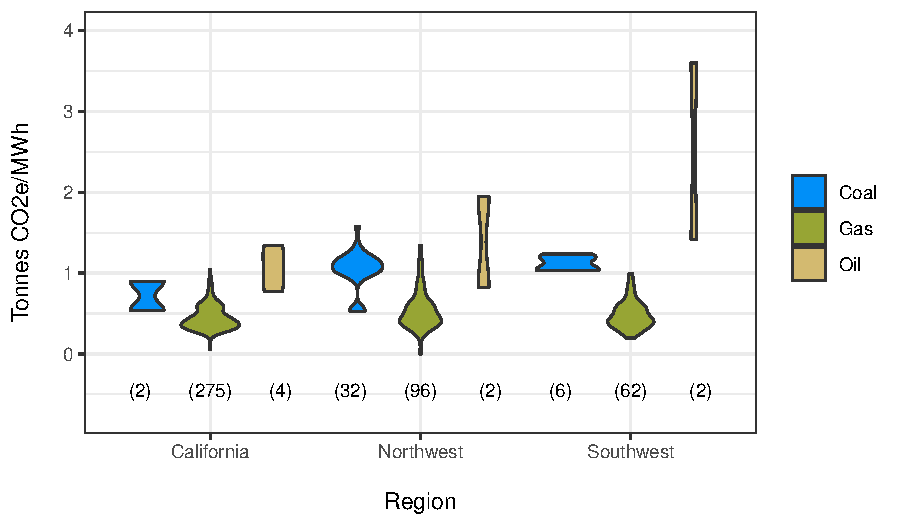
\includegraphics[width=0.8\textwidth]{figures/chapter5_figures/EI_region_violin.pdf}
    \fignote[1]{
        Figure displays the distribution of greenhouse gas emissions intensities by region and fuel type. Emissions intensities are measured in tonnes of carbon dioxide equivalent (CO$_2$e) per megawatt-hour (MWh). For context, the average monthly US household electricity consumption was 0.886 MWh of electricity in 2021. The number of generators in group is displayed below the violinplot in parentheses. 
    }
\end{figure}

The violinplots in Figure \ref{ghg_intensity} display the distribution of greenhouse gas emissions intensities (CO$_2$e/MWh) by region and fuel. These emissions intensities are calculated by multiplying the emissions intensity of the specific variety of fuel a generator uses, measured in CO$_2$e/MMBtu, and multiplying it by the generator's heat rate, measured in MMBtu/MWh. The number of generators in each region and with each fuel is below the violinplot in parentheses. Overall, this shows that gas generators generally have the lowest greenhouse gas emissions intensities. In both the Northwest and Southwest, gas power plants are almost always less emissions intensive than coal and oil power plants. In California, coal, gas, and oil generators have similar emissions intensities, likely a result of regulation that has forced the closure of less efficient coal and oil power plants. Oil generators in general have the greatest spread in emissions intensities. 

\begin{figure}
    \centering
    \caption{Local Air Pollutant Emissions Intensities by Fuel\label{pol_intensities}}
    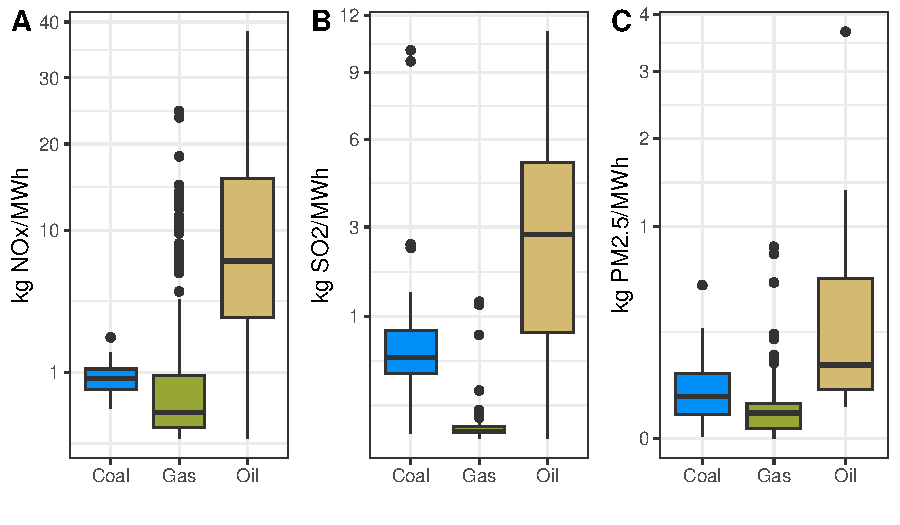
\includegraphics[width=0.8\textwidth]{figures/chapter5_figures/local_poll_EI.pdf}
    \fignote[1]{
        Figure displays the distribution of criteria air pollutant emissions intensities by generator fuel type. Panel A, B, and C visualize these the distributions of nitrogen oxides (NO$_x$), sulfur dioxide (SO$_2$), and fine particulate matter (PM2.5). These distributions are highly right skewed, so the vertical axis in each panel uses a squareroot transformation. 
    }
\end{figure}

Figure \ref{ghg_intensity} demonstrates that while there is some variation in the greenhouse gas emissions intensities of generators across the different regions and fuels, these distributions are fairly close to each other. This is not the case for local air pollutant emissions intensities. Figure \ref{pol_intensities} displays these distributions for each of the three local air pollutants, NO$_x$, SO$_2$, and PM2.5, for generators of each fuel category. First note that all figures use a squareroot scale on the vertical axis so these distributions are clearer to see. For each pollutant, gas generators have the lowest median emissions intensity, coal the second lowest, and oil highest. Gas generators create essentially no SO$_2$ emissions, but it is not uncommon for gas generators to have just as high NO$_2$ emissions intensities as coal generators. Oil generators are again highly variable, sometimes varying my an order of magnitude. 

Lastly, I augment the power plant data with data on the appropriate fuel prices. Power plants report their fuel costs on a regular basis (frequency depends on the fuel) as a part of Form EIA-860. The EIA reports these prices at the state level, so I aggregate these to get region-specific prices for coal and gas for power plants. There are so few power plants that continue to fuel oil that the EIA does not report the prices these power plants pay for fuel oil for data confidentiality. Instead, I use the price of West Texas Intermediate Crude oil out of Cushing, Oklahoma (the standard quote price for oil) reported by the EIA. The analysis will use time-invariant fuel prices, so I average prices over the relevant timeframe, and make the necessary conversions to get the price of each generator pays for fuel in USD/MMBtu. Additional details on the fuel prices appear in Appendix A.5 with Figures and Table \ref{fuel_prices}.

With the complete set of power plants, I implement the $k$-means clustering algorithm as described in the previous section to group these power plants together into thirty representative power plants. Clustering groups the power plants together based on their nameplate capacity and their heat rate. This distribution of the capacities and heat rates for power plants in these groups is given in Figures \ref{cluster_cap} and \ref{cluster_hrate} in Appendix A.5. 

\subsubsection*{Electricity Demand}

Regional electricity demand data come from the EIA's Hourly Electric Grid Monitor---Region files. These files report the total electricity demand in each region at every hour, and beginning in July of 2018, report the fuel source used to meet this demand. For each hour between the start of 2019 through 2021, I find the residual electricity demand in each region by taking the total demand and subtracting generation from all fuel sources other than coal, gas, and oil. I link the residual demand in each region for each hour in the time period, and then perform $k$-means clustering to identify twenty-four representative hours. 

Electricity demand has strong temporal patterns, both trends within a day and seasonal trends that unfold over the course of the year. Figures \ref{hourly_demand} and \ref{monthly_demand} in Appendix A.5 display these temporal patterns for the entire Western Interconnection. 

\begin{figure}
    \centering
    \caption{Distribution of Residual Demand by Region\label{dist_rdemand}}
    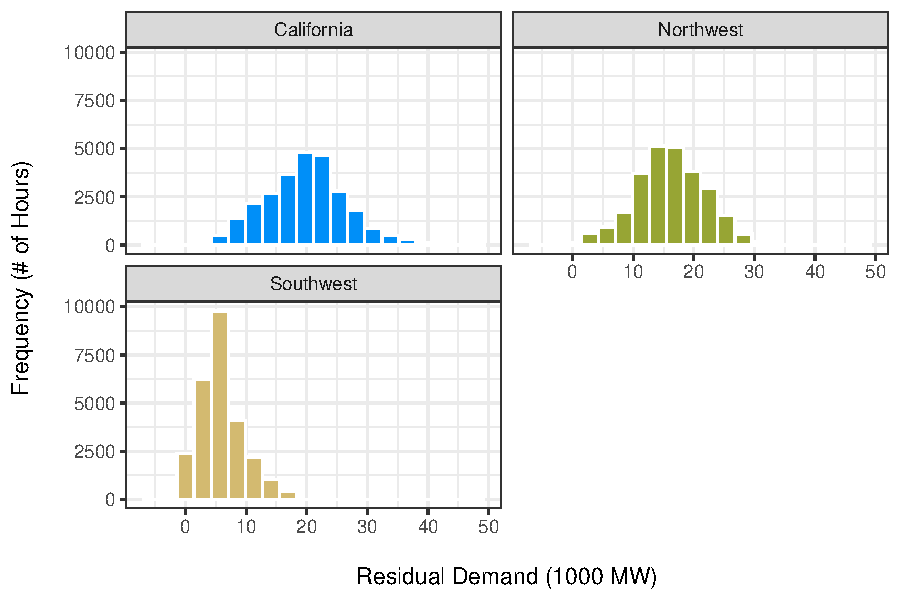
\includegraphics[width=\textwidth]{figures/chapter5_figures/residual_demand_region.pdf}
    \fignote[1]{
        Figure displays the distribuition of residual demand for each region. Frequencies describe the number of hours in the three year period from 2019--2021 with residual demand values within the given bin. Note that California is the region with the highest average residual electricity demand, and although it is difficult to see on the figure, also the region with the most variance in residual electricity demand.
    }
\end{figure}

Recall from Chapter 4 that the transmission constraints require a designated ``swing hub." In this analysis, I designate California as the swing hub, a decision guided by Figure \ref{dist_rdemand}. The swing hub is an important  reference point for all interregional transmission, and the marginal power injections in the all other regions presumably flow to or through the swing hub. Figure \ref{dist_rdemand} demonstrates that California has the greatest average residual demand, but from Figure \ref{generators_dist}, it is clear that California does not have the greatest residual capacity (coal + gas + oil capacity) and consequently will be the mostly likely to import electricity. Although it is not a requirement for the swing hub to consistently import electricity from the other regions, it does aid in the interpretation of the transmission constraint. Additional data related to the transmission constraints come from the dataset used in \cite{fowlie2021border}. 

\subsubsection*{Disadvantaged Communities}

Lastly, analyzing the effect of carbon pricing on air pollution concentration in disadvantaged communities relative to non-disadvantaged communities requires designated disadvantaged and non-disadvantaged communities. 
As mentioned when reviewing the empirical strategy of the simulation, the original dichotomization of this variable and the terminology itself stems from California State Bill 535. Like many jurisdictions with a carbon price, California requires that some of the funds raised through emissions allowance auctions be directed back to those people most exposed to climate change and environmental risks broadly. California SB 535 specifies this, requiring a proportion of the funds raised to go back to ``disadvantaged communities.'' The California EPA is responsible for determining what areas are considered to be disadvantaged under the bill. To define each community,  California EPA uses 2010 Census tracts. From there, regulators create an index that combines measures of environmental degradation in the Census tract and measures of population sensitivity to environmental degradation. The current version of this index is called CalEnviroScreen 4.0. 

According to \cite{oehha2022sb}, a Census tract is assigned Disadvantaged Community (DAC) status if at least one of the following criteria is met: 
\begin{enumerate}
    \item The Census tract ranks in the top 25\% of all Census tracts in California on the CalEnviroScreen 4.0 index. 
    \item The Census tract has missing data, but ranks in the top 5\% of Census tracts in California based on its pollution burden subindex.
    \item The Census tract was designated as a DAC at the time of last review (2017).
\end{enumerate}
In addition to these conditions, other communities that are not necessarily Census tracts are eligible for DAC status if a federally recognized Tribe establishes that the land is under its control. 

Although the DAC designation under SB 535 is a useful benchmark for Census tracts in California, Census tracts outside of the state do not have a DAC designation, and the geography of interest in includes many of these communities. To overcome this issue, I use data from the US EPA's Environmental Justice Screening tool to replicate the CalEnviroScreen 4.0 index on all Census tracts in the Western Interconnection. I begin by identifying all 2010 Census tracts located in the Western Interconnection using shapefiles of both 2010 Census tracts and the shapefile for the Western Interconnection. Then I crosswalk the variables that make up CalEnviroScreen 4.0 with variables in the EPA's Environmental Justice Screening tool and use these variables to reconstruct an index analogous to CalEnviroScreen 4.0. Details of the variable crosswalk between the CalEnviroScreen dataset and the EPA's Environmental Justice screening dataset as well as details on the index calculation appear in Appendix A.5. Following the analogous criteria for DAC designation and the reconstructed index that has observations for all Census tracts in the study geography, I then classify each Census tract in the Western Interconnection as either ``Disadvantaged'' or ``Non-disadvantaged.'' The specific criteria for DAC status in the reconstructed measure are:
\begin{enumerate}
    \item The Census tract ranks in the top 25\% of all Census tracts in Western Interconnection based on the reconstructed index.
    \item The Census tract has missing data, but ranks in the top 5\% of Census tracts in the Western Interconnection based on the reconstructed index. 
    \item The Census tract overlaps with an official unit of Tribal land that is at least ten square miles in area.\footnote{For this, I use the US Census Bureau's 2021 shapefile of Tribal Census tracts. The stipulation that each unit of the Tribal land must be at least ten square miles in area prevents Census tracts with very small areas of land owned by Tribes from automatically receiving DAC status when this land is not lived on or lived on by very few people.}
\end{enumerate}
Apart from the difference in the index itself, the criteria for DAC designation in this study differs from the original criteria for DAC designation in several substantive ways. First and most importantly, DAC designation based on the percentile ranking of the reconstructed index includes all Census tracts in the Western Interconnection, not just those in California. This means that is now possible for more than (or less than) 25\% of Census tracts in California to meet the first criterion and be designated as a DAC. The same ranking difference applies to the second criterion as well. These criteria also do not contain a simulation that Census tracts designated as DAC under the previous version of CalEnviroScreen receive DAC designation in the current version. This criterion is excluded primarily because there is no data available for this period, but ultimately this is not a significant concern as only nineteen Census tracts had DAC status in the previous version of CalEnviroScreen but would otherwise not have been designated DAC if it were not for this stipulation. 

\begin{figure}
    \centering
    \caption{Disadvantaged Communities (DACs) Designation Comparison \label{sb535_comp}}
    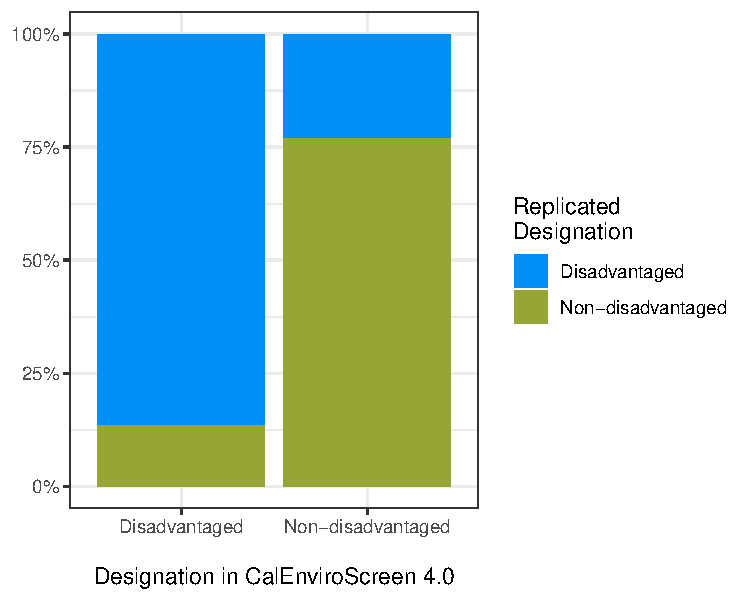
\includegraphics[width=0.7\textwidth]{figures/chapter5_figures/DAC_designation.pdf}
    \fignote[.9]{
        Figure compares the reconstructed DAC designations for Census tracts in California and the  official DAC designations under CalEnviroScreen 4.0. Most all (87.8\%) of Census tracts officially classified as DACs in California are also classifed as DACs by the reconstructed index and criteria. It is not uncommon (24.9\%) for Census tracts that are not officially classified as DACs to be classified as a DAC in the reconstructed designation. 
    }
\end{figure}

The goal of reconstructing the CalEnviroScreen index is to create a designation analogous to California's DAC designation that is available across the entire Western Interconnection. Although this is not the same as creating a designation for all Census tracts in the Western Interconnection that identically matches California's designation, ideally the reconstructed DAC designation would identify many of the same communities that have been officially identified under SB 535. Figure \ref{sb535_comp} compares the reconstructed or replicated designation of a DAC to the official designation of a DAC for 2010 Census tracts in California. The reconstructed DAC designation correctly identifies the majority of official DACs---87.8\% of Census tracts officially designated as DAC are also designated as DAC under the reconstructed designation. It is more common for a Census tract that is not officially designated as a DAC to be designated as a DAC in the reconstructed measure---24.9\% of Census tracts that are not officially designation as DAC are designated as DAC under the reconstructed designation. This is likely because across the Western Interconnection, many communities in California have greater pollution burdens and more sensitive populations than communities in other states, like Idaho or Utah. Adding in more communities with low scores in the index allows communities in California that previous fell short of the DAC designation to become eligible. Table \ref{dac_summary} in Appendix A.5 compares summary statistics for disadvantaged and non-disadvantaged communities across the Western Interconnection.

\subsection{Results}

This section presents the results of the policy simulations outlined in Table \ref{policy_scenarios} that use the data discussed in the previous section. The simulation model creates predictions along five different dimensions: generation, investment, greenhouse gas emissions, local air pollutant emissions, and the EI Gap. Because California does have a border carbon adjustment (BCA) for the electric power industry, unless stated otherwise, the results in this section focus on just those policy scenarios with a BCA. Results for policy simulations without a BCA appear in Appendix A.5.

\subsubsection*{Generation}

Electricity demand is assumed to be perfectly inelastic, such that increases in wholesale electricity prices under the cap-and-trade program will not lead to changes in the quantity of electricity demanded. This means that the carbon price will have no effect on the quantity of electricity generated, but still could affect the composition of generation. 

% Figure \ref{}

% \begin{figure}
%     \centering
%     \caption{\label{}}
%     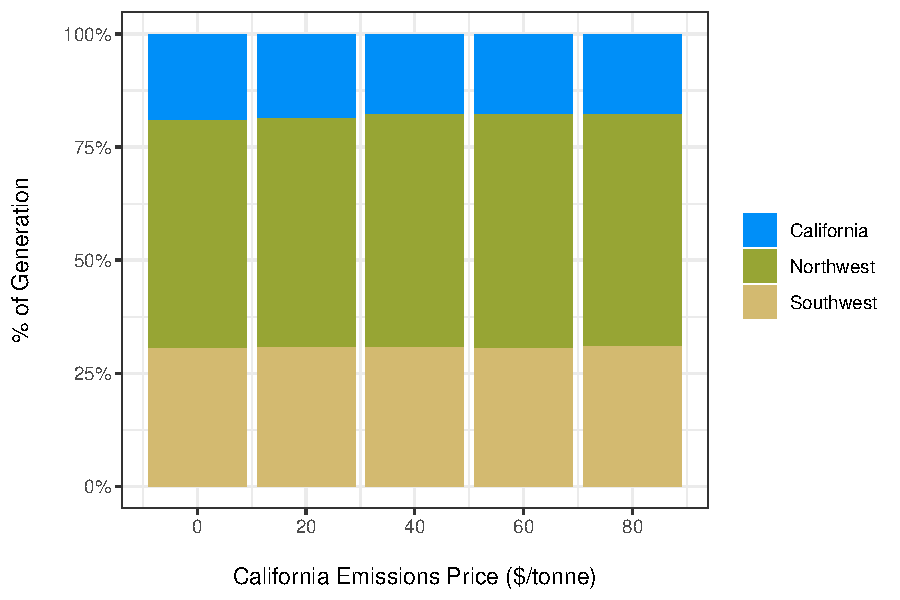
\includegraphics[width=0.8\textwidth]{figures/chapter5_figures/gen_region_bca.pdf}
%     \fignote[1]{
%         Figure shows\ldots
%     }
% \end{figure}

In the simulation with a BCA, raising the carbon price has essentially no effect on the distribution of generation across the three regions. The raising the carbon price in California from \$0 to \$80 lowers California's domestic generation by only 7.25\%. Again, demand is fixed so all generation forgone in California is just replaced by generation in the other two regions. About two-thirds (67.8\%) of the generation forgone in California moves to the Northwest, and the remaining third (32.2\%) of generation moves to the Southwest. In the absence of a BCA, much more generation shifts outside of California. Raising the carbon price in California from \$0 to \$80 lowers California's domestic generation by 16.3\%. 

\begin{figure}
    \centering
    \caption{Simulated Fuel Composition of Generation \label{gen_fuel_bca_pct}}
    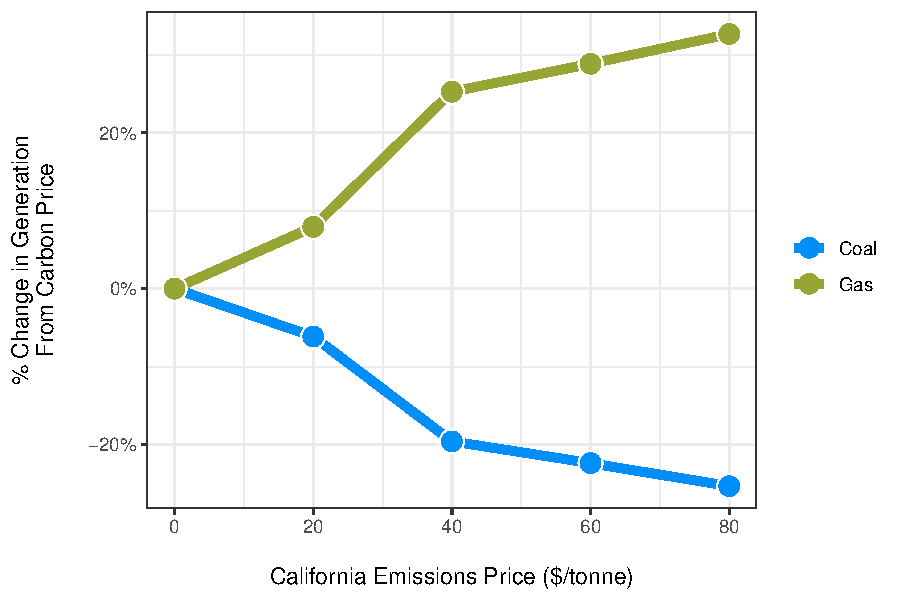
\includegraphics[width=0.8\textwidth]{figures/chapter5_figures/gen_fuel_bca_pct.pdf}
    \fignote[.9]{
        Figure shows the percent change in annual generation for coal and gas attributable to the carbon price from the baseline scenario where the carbon price is zero. This simulation uses a BCA. This includes all generation across the Western Interconnection.
    }
\end{figure}

More interesting---and relevant for the environmental implications of the policy---is the effect of the carbon price on the fuel composition of the electricity generation. Figure \ref{gen_fuel_bca_pct} visualizes how the composition of fossil fuel generation changes as a result of the carbon price. First note that in the policy simulations, there is no generation from oil. This is not surprising as there is little capacity from oil power plants and as oil is consistently the most expensive fuel. Empirically, oil power plants generally have a very low capacity factor, meaning that they rarely operate. Second, notice that increasing the carbon price has the effect we would expect based on the emission intensities of different types of power plants in Figure \ref{ghg_intensity}. As the carbon price increases, generation shifts away from the more CO$_2$e intensive coal power plants and towards the less CO$_2$e intensive gas power plants. 

% Put these next two in the appendix for sure

% \begin{figure}
%     \centering
%     \caption{\label{}}
%     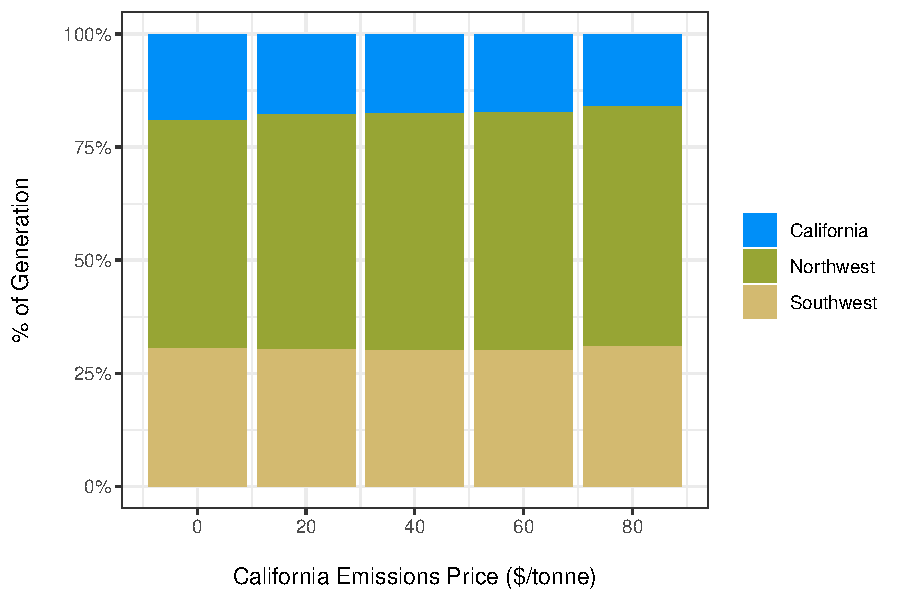
\includegraphics[width=0.8\textwidth]{figures/chapter5_figures/gen_region_nobca.pdf}
%     \fignote[1]{
%         Figure shows\ldots
%     }
% \end{figure}

% \begin{figure}
%     \centering
%     \caption{\label{}}
%     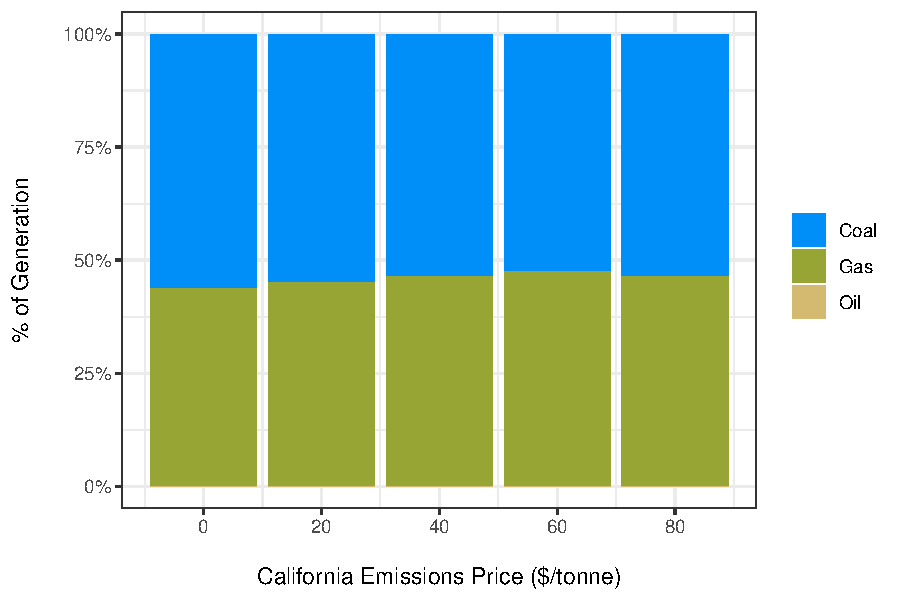
\includegraphics[width=0.8\textwidth]{figures/chapter5_figures/gen_fuel_nobca.pdf}
%     \fignote[1]{
%         Figure shows\ldots
%     }
% \end{figure}

\subsubsection*{Heat Rate Improvements}

In the simulation, power plants have the option to invest in a heat rate improvement. Recall that to simplify the simulation, I split all generators into four groups: two groups from California and two groups from outside of California. Figure \ref{inv_region} plots the number of power plants that invest in heat rate improvements under each value of the carbon price. At a carbon price of \$0 per tonne CO$_2$e, a small group of power plants from California and all power plants outside of California invest in heat rate improvements. As the carbon price increases to \$20 per tonne CO$_2$e, all power plants in the Western Interconnection make heat rate improving investments. 

\begin{figure}
    \centering
    \caption{Power Plants Making Heat Rate Improving Investments \label{inv_region}}
    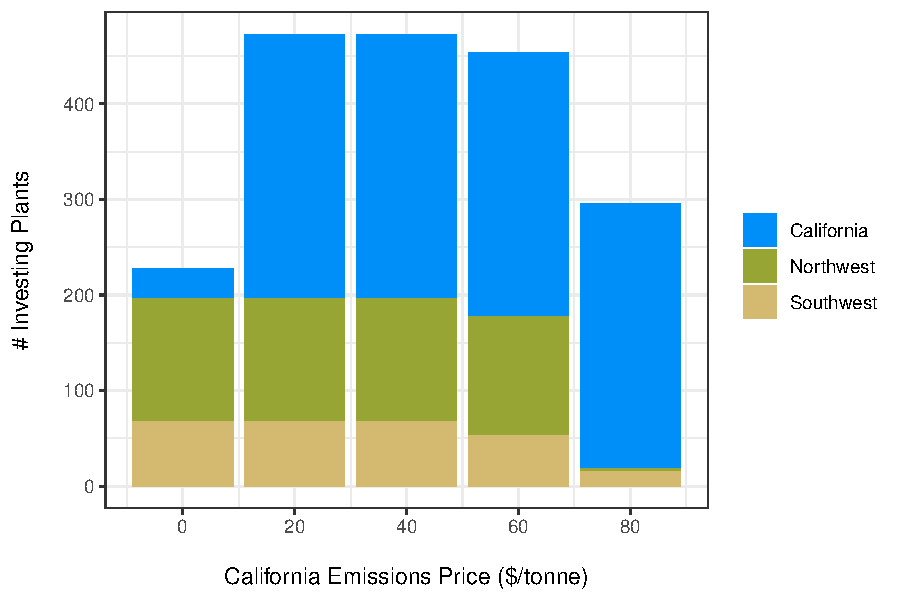
\includegraphics[width=0.8\textwidth]{figures/chapter5_figures/inv_region.pdf}
    \fignote[.9]{
        Figure shows the number of power plants that make heat rate improving investments under each carbon price. All policy scenarios in the figure include a BCA. 
    }
\end{figure}

Given that all power plants outside of California are willing to make heat rate improving investments even when there is no price on carbon, there is some concern that the parameters in the investment cost function from \cite{weber2021dynamic} do not generalize well to power plants outside of the state. To accommodate this concern, I also simulate all policy scenarios with a high investment cost scenario, where all investment costs are increased by an order of magnitude. In these simulation results, which appear in Figure \ref{hc_inv_region} in Appendix A.5, only one group of power plants in California and one group of power plants outside of California are willing to invest in heat rate improvements when the price of carbon is \$20 per tonne of CO$_2$e or less. At prices of \$40 per tonne of CO$_2$e and greater, all power plants invest in heat rate improvements. That is, raising the carbon price in California induces investment in heat rate improvements for fossil fuel power plants even outside of the state. This is only true in the case where California implements a BCA; otherwise, California's carbon price does not induce power plants outside of the state to invest in heat rate improvements.

Admittedly, the investment profiles are crude and the investment cost estimates are not convincing for this application. Still, the magnitude of these heat rate improvements is small (1.5\%), so it is unlikely that heat rate improvements will significantly affect the primary results related to the EI Gap. Importantly though, the high investment cost simulations demonstrate that, when coupled with a BCA, unilateral carbon pricing has the potential to induce efficiency investments in regions that are not covered by the carbon price. 

\subsubsection*{Greenhouse Gas Emissions}

The primary objective of a carbon price is to reduce greenhouse gas emissions, so while this analysis does not focus on evaluating the potential of carbon pricing to reduce greenhouse gas emissions, the effect of carbon pricing on greenhouse gas emissions is still central. Before reviewing the simulation results though, consider first the mechanisms in the model through which greenhouse gas emissions could occur. Again, demand is inelastic, so emissions reductions cannot occur as a result of reductions in the total quantity of electricity generated. Investment has a limited potential to affect emissions as the model does not occupy a long enough time frame to consider investments in alternative sources of electricity, but existing power plants have a small capacity to reduce their emissions through efficiency improvements. The main mechanism for reducing greenhouse gas emissions is then just by reallocating generation to power plants that are less emissions intensive. 

Figure \ref{sim_co2e_bca} demonstrates that this mechanism is able to create emissions reductions in the short run. Without a carbon price, total greenhouse gas emissions from electric power generation in the Western Interconnection is about 289 million tonnes CO$_2$e each year. Implementing a carbon price of \$80 per tonne though reduces total greenhouse gas emissions by 11.90\% or 33.7 million tonnes CO$_2$e annually---the equivalent of removing 7.3 million passenger cars from the road. 

\begin{figure}
    \centering
    \caption{Simulated Greenhouse Gas Emissions\label{sim_co2e_bca}}
    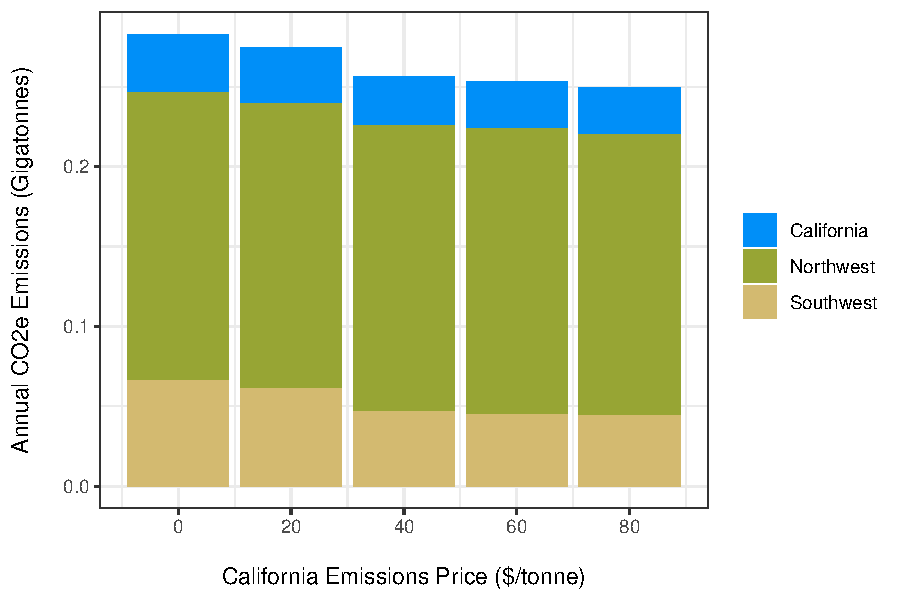
\includegraphics[width=.9\textwidth]{figures/chapter5_figures/sim_co2e_bca.pdf}
    \fignote[.9]{
        Panel A of the figure displays the simulated greenhouse gas emissions from electric power generation across the Western Interconnection. Panel B of the figure displays the simulated changes in greenhouse gas emissions from the baseline scenario where there is no carbon price. All simulations contain a BCA. 
    }
\end{figure}

Note also the distribution of these emissions reductions across the three regions. The \$80 carbon price causes 20.3\%, 2.1\%, and 33.8\% emissions reductions from electric power generation in California, the Northwest, and the Southwest respectively. This is rare instance of negative leakage, where the implementation of a unilateral carbon price actually causes emission reductions in jurisdictions that do not face the carbon price. Because California imports much of their electricity and the BCA gives preference to cleaner domestic electricity generation, then the Northwest and Southwest see emissions reductions as well. 

\begin{figure}
    \centering
    \caption{Simulated Greenhouse Gas Emissions---No BCA\label{sim_co2e_nobca}}
    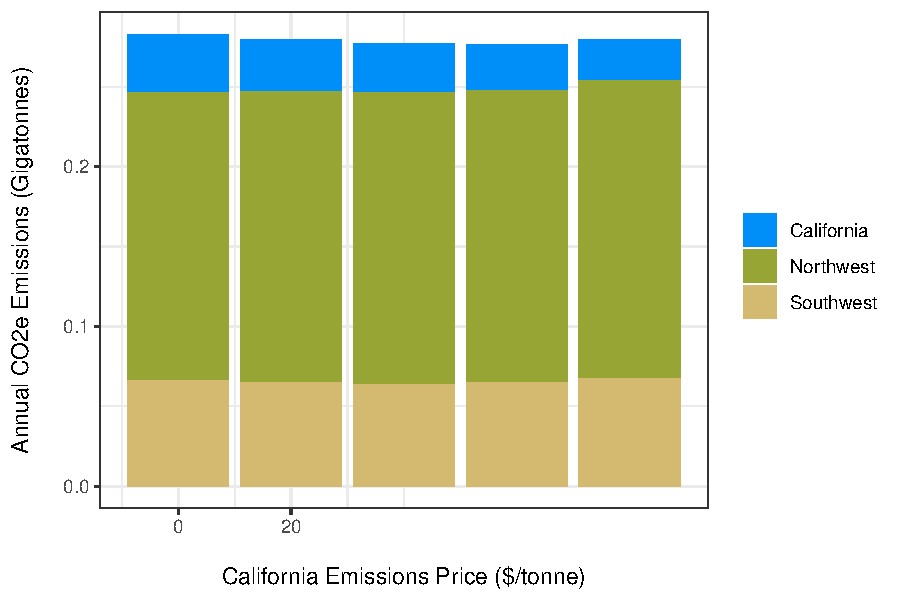
\includegraphics[width=0.8\textwidth]{figures/chapter5_figures/sim_co2e_nobca.pdf}
    \fignote[.9]{
        Panel A of the figure displays the simulated greenhouse gas emissions from electric power generation across the Western Interconnection. Panel B of the figure displays the simulated changes in greenhouse gas emissions from the baseline scenario where there is no carbon price. Simulations do not contain a BCA.
    }
\end{figure}

Figure \ref{sim_co2e_nobca} displays the impact of the carbon price on greenhouse gas emissions without a BCA. In this case, California experiences a more dramatic 28.8\% reduction in its own greenhouse gas emissions under a \$80 carbon price, but both the Northwest and Southwest increase their emissions by 3.7\% and 1.1\% respectively. Additionally, greenhouse gas emissions are not monotonically decreasing in the carbon tax in the absence of a BCA. Of the carbon prices considered, the lowest greenhouse gas emissions are achieved at a carbon price of \$60. These emissions reductions are far more modest though, only amounting to a 2.4\% decrease in emissions across the Western Interconnection.\footnote{The leakage rate is a common metric used to assess the impact of BCAs and is calculated as the ratio of foreign emissions increases to domestic emissions reductions. With a carbon price of \$80 per tonne CO$_2$e, there is a leakage rate of 70.2\% without a BCA and a leakage rate of -354\% with a BCA.}

\subsubsection*{Local Air Pollution Emissions}

Co-pollutants---including nitrogen oxides, sulfur dioxide , and fine particulate matter---all see similar changes to greenhouse gas emissions under the carbon price. Simulated levels and changes in the levels of these three local air pollutants are shown appear in Figure \ref{sim_pol_bca}. 

\begin{figure}
    \centering
    \caption{Simulated Local Air Pollution Emissions\label{sim_pol_bca}}
    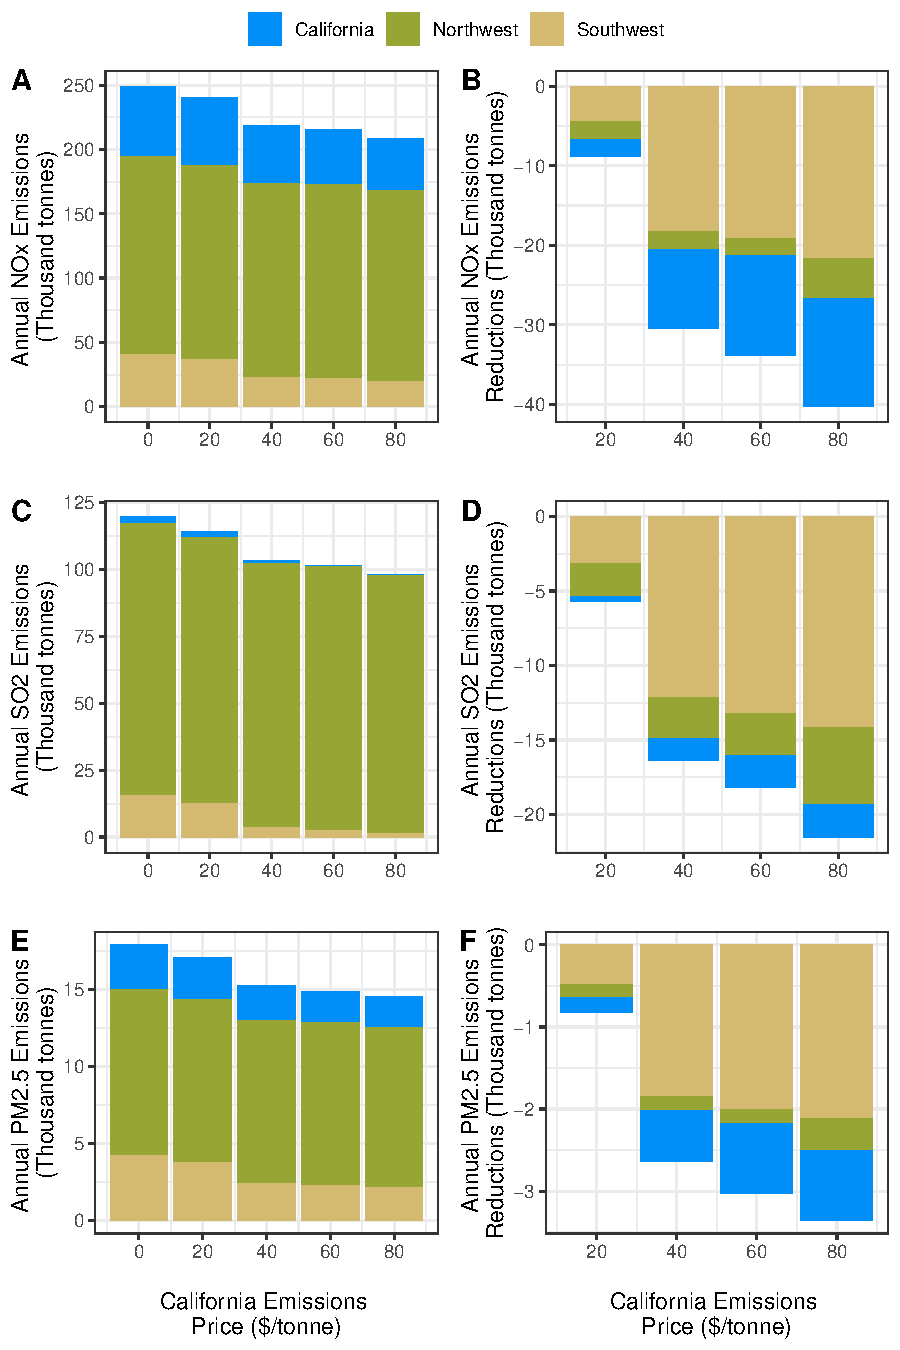
\includegraphics[width=0.8\textwidth]{figures/chapter5_figures/sim_pol_bca.pdf}
    \fignote[1]{
        Figure displays the simulated impact of carbon pricing on emissions of three local air pollutants: nitrogen oxides (NO$_x$), sulfur dioxide (SO$_2$), and fine particulate matter (PM2.5). 
        Panels A, C, and E visualize the total levels of these emissions, and Panels B, D, and F display the changes in these emissions from the baseline scenario where there is no carbon price. All simulations include a BCA. 
    }
\end{figure}

Nitrogen oxides (NO$_x$) are the primary air pollutant of concern in electric power generation. By tonnes, power plants create more NO$_x$ emissions than emissions of any of other local air pollutant. In addition to being relatively more common, NO$_x$ emissions are also more ubiquitous in electric power generation. This is not the case with sulfur dioxide (SO$_2$) which is released almost exclusively by coal-fired power plants. Regulators and generator owners make plans to retire coal-fired power plants, these SO$_2$ emissions from electric power generation will largely subside, but NO$_x$ emissions will not. Fine particulate mater (PM2.5) is also a serious concern, but PM2.5 emissions generally come from sources other than electric power generation, especially personal vehicles. 

Figure \ref{sim_pol_bca} demonstrates that the carbon price in California leads to consistent and substantive emissions reductions across the entire Western Interconnection. The Southwest region makes the largest contributions to these emissions reductions---a consequence of the region's relatively dirty power plants and the trade exposure of the region's fossil-fueled power plants. California's fossil fuel power plant fleet is largely made up of gas generators rather than coal, so California makes only modest reductions in SO$_2$ emissions under the carbon price, but notable reductions in NO$_x$ and PM2.5 emissions. Overall though, the carbon price is able to not only reduce greenhouse gas emissions, but emissions of local co-pollutants as well. 




% \begin{figure}
%     \centering
%     \caption{\label{}}
%     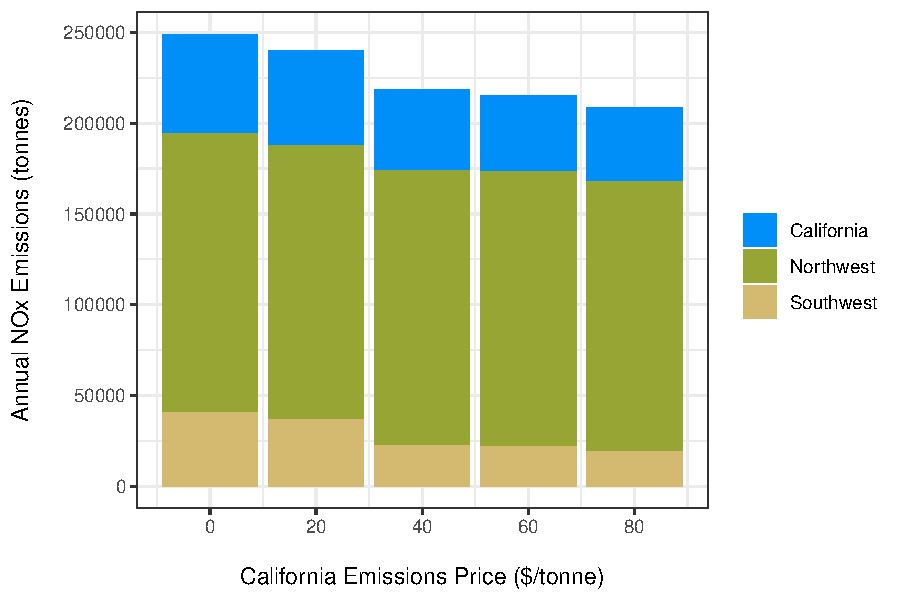
\includegraphics[width=0.8\textwidth]{figures/chapter5_figures/sim_nox_bca.pdf}
%     \fignote[1]{
%         Figure shows\ldots
%     }
% \end{figure}

% \begin{figure}
%     \centering
%     \caption{\label{}}
%     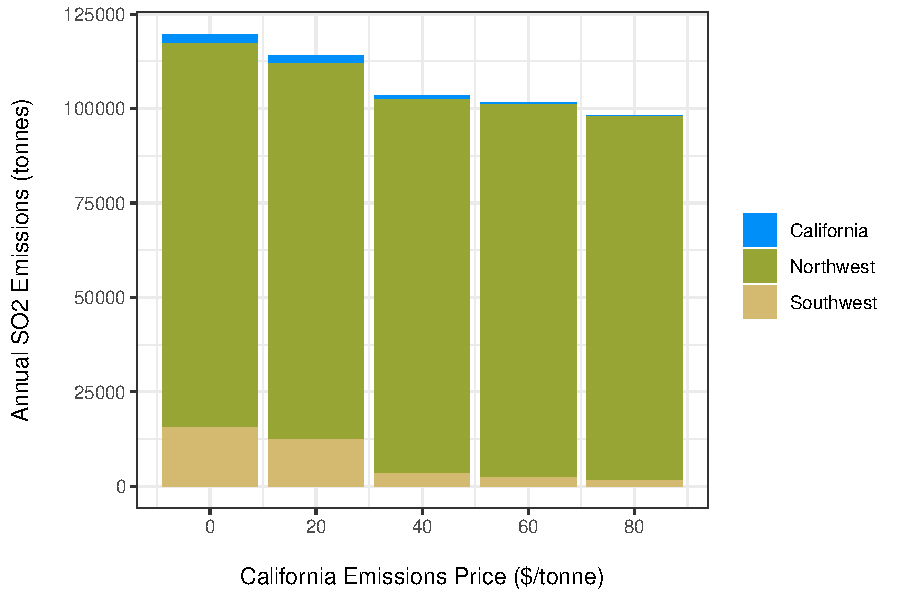
\includegraphics[width=0.8\textwidth]{figures/chapter5_figures/sim_so2_bca.pdf}
%     \fignote[1]{
%         Figure shows\ldots
%     }
% \end{figure}

% \begin{figure}
%     \centering
%     \caption{\label{}}
%     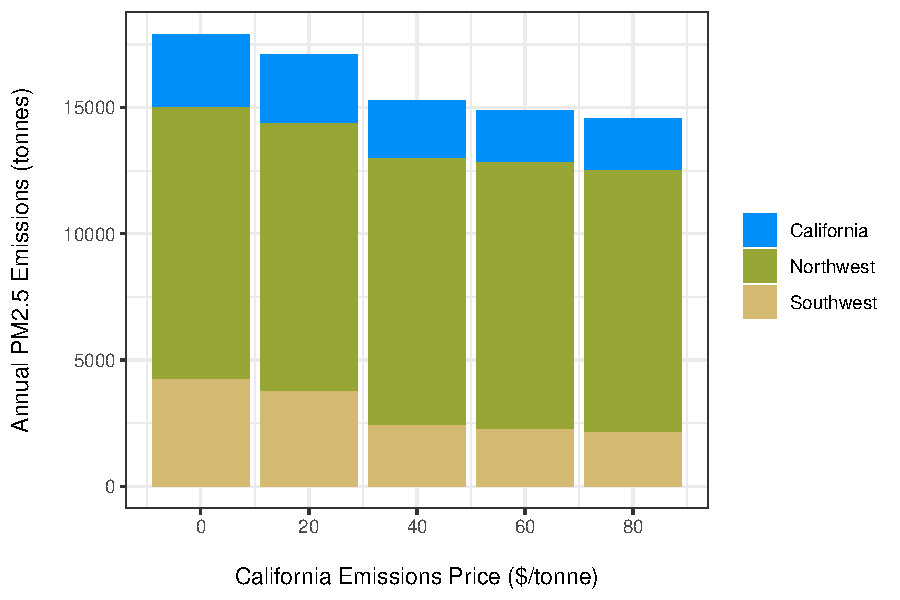
\includegraphics[width=0.8\textwidth]{figures/chapter5_figures/sim_pm25_bca.pdf}
%     \fignote[1]{
%         Figure shows\ldots
%     }
% \end{figure}





% % Add to the appendix (maybe later)

% \begin{figure}
%     \centering
%     \caption{\label{}}
%     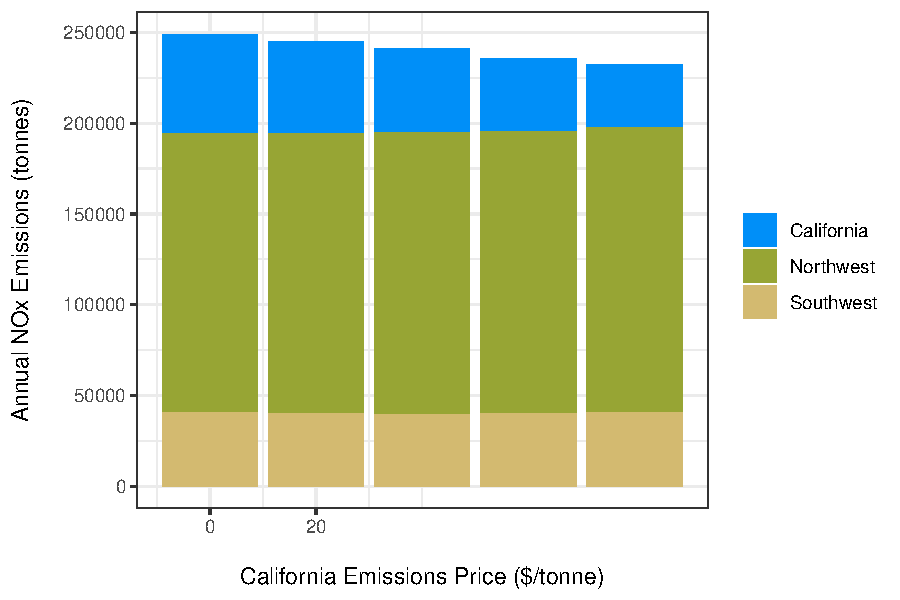
\includegraphics[width=0.8\textwidth]{figures/chapter5_figures/sim_nox_nobca.pdf}
%     \fignote[1]{
%         Figure shows\ldots
%     }
% \end{figure}

% \begin{figure}
%     \centering
%     \caption{\label{}}
%     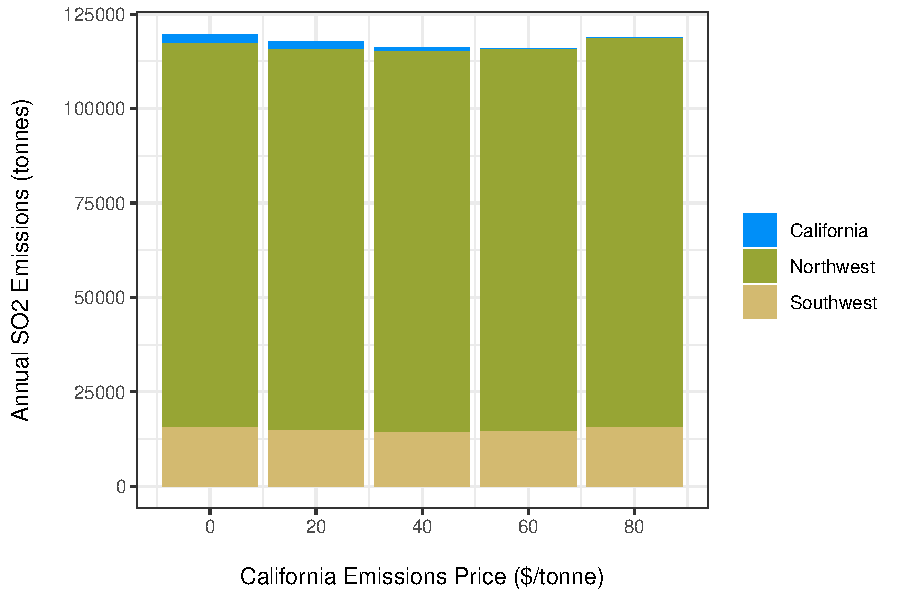
\includegraphics[width=0.8\textwidth]{figures/chapter5_figures/sim_so2_nobca.pdf}
%     \fignote[1]{
%         Figure shows\ldots
%     }
% \end{figure}

% \begin{figure}
%     \centering
%     \caption{\label{}}
%     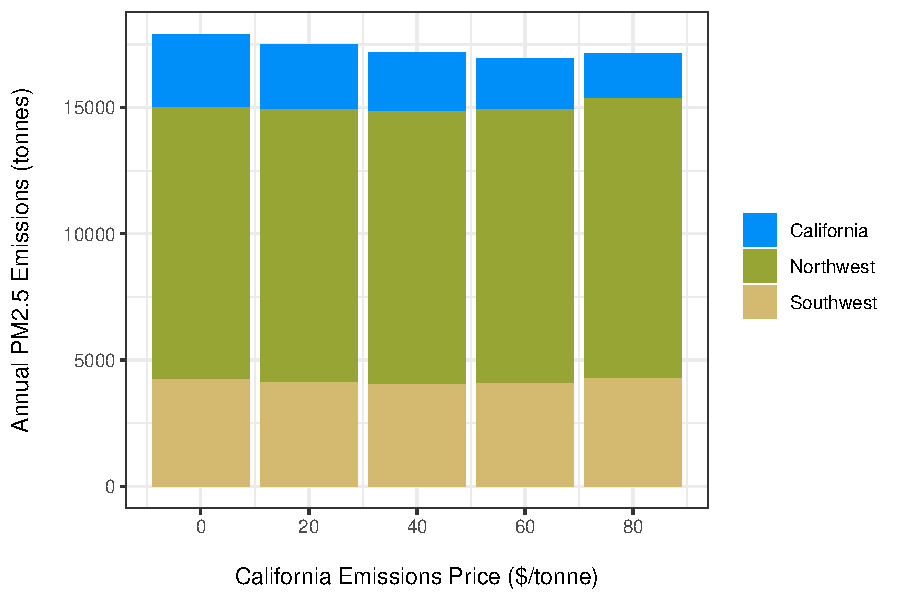
\includegraphics[width=0.8\textwidth]{figures/chapter5_figures/sim_pm25_nobca.pdf}
%     \fignote[1]{
%         Figure shows\ldots
%     }
% \end{figure}

\subsubsection*{The Environmental Inequality Gap}

The primary objective of the text overall is to assess the effects of carbon pricing on environmental inequalities. In particular, the paper has focused on the potential or lack thereof for carbon pricing to exacerbate disparities in air pollution concentration between disadvantaged communities (DAC) and non-disadvantaged communities (non-DAC). Chapter 4 developed a measurement of these disparities that I have called the Environmental Inequality Gap or EI Gap. The EI Gap is simply the difference in the average concentration of an air pollutant in a DAC and the average concentration of this air pollutant in a non-DAC, where the air pollution under consideration is just that air pollution associated with electric power generation. This subsection proceeds by reviewing the simulation results of the EI Gap for the three co-pollutants under consideration, and then attempts to make sense of these results in light of the intuition provided by the model.

First consider the EI Gap for nitrogen oxides. Figure \ref{ei_gap_bca_nox} visualizes the EI Gap for nitrogen oxides across the Census tracts in the Western Interconnection. The blue series represents the average concentration of NO$_x$ emissions in DACs at each level of the carbon price, and the green series represents te average concentration of NO$_x$ emissions in non-DACs at each level of the carbon price. The difference between the blue and green series is the value of the EI Gap. Note first that for NO$_x$, this gap is positive, indicating that even in the baseline case where there is no carbon price, that DACs experience a higher concentration of NO$_x$ pollution than non-DACs in the Western Interconnection. Crucially though, this figure reveals a necessary and important truth: raising the carbon price increases the EI Gap. Not only does the figure show that the EI Gap for NO$_x$ emissions increases in the carbon pricing, it also demonstrates that the concentration of NO$_x$ could plausibly increase in DACs when faced with a carbon price. 

\begin{figure}
    \centering
    \caption{The EI Gap for NO$_x$ \label{ei_gap_bca_nox}}
    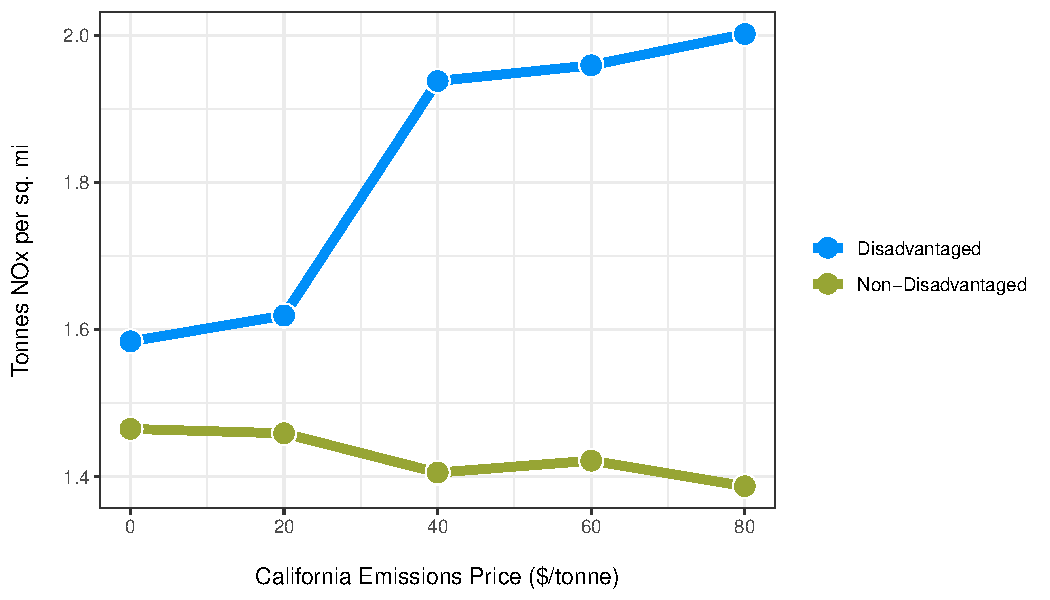
\includegraphics[width=0.7\textwidth]{figures/chapter5_figures/ei_gap_bca_nox.pdf}
    \fignote[.8]{
        The figure demonstrates that, yes, it is possible for a unilateral carbon price will increase air pollution in DACs. Figure shows the simulated average concentration of NO$_x$ for DACs and non-DACs across five different carbon prices for all Census tracts in California. The distance between the two series is the EI Gap. 
    }
\end{figure}

Why does the EI Gap increase for NO$_x$ in the policy simulation, and why does the concentration of NO$_x$ increase for DACs? Recall from Chapter 4 that there are two primary mechanisms through which raising the carbon price could affect the EI Gap. The first of these mechanisms was the emissions intensity mechanism: if power plants in and around DACs have lower CO$_2$e emissions intensities at the margin than power plants in and around non-DACs, then an increase in the carbon price can widen the EI Gap. The second of these mechanisms is related to the multiregion nature of the model: if power plants in and around DACs face a lower carbon price than power plants in and around non-DACs, then an increase in the carbon price can widen the EI Gap. 

\begin{figure}
    \centering
    \caption{The EI Gap for NO$_x$ in California \label{ei_gap_bca_nox_cal}}
    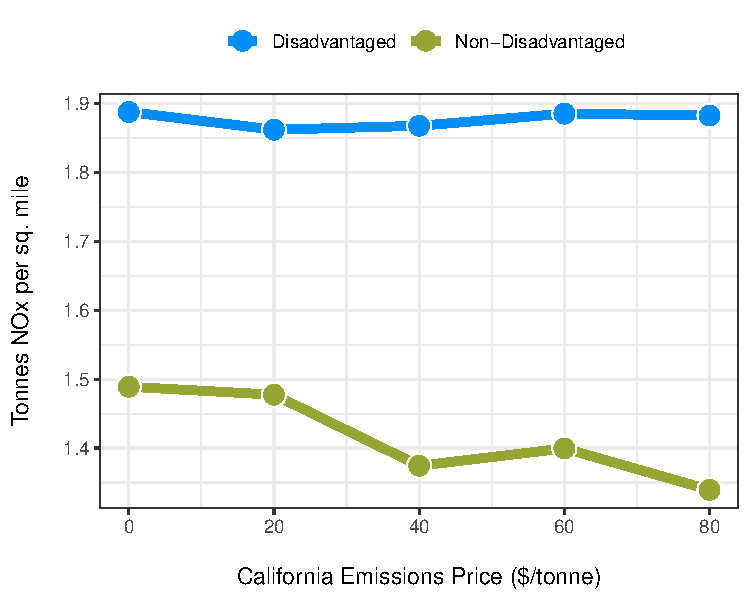
\includegraphics[width=0.7\textwidth]{figures/chapter5_figures/ei_gap_bca_nox_cal.pdf}
    \fignote[.8]{
        Figure shows the simulated average concentration of NO$_x$ for DACs and non-DACs across five different carbon prices for the subset of Census tracts in California. The distance between the two series is the EI Gap. Although the EI Gap is clearly widening under the carbon price, this widen is much more extreme when all Census tracts are considered. 
    }
\end{figure}

Paired with the logic above, Figure \ref{ei_gap_bca_nox_cal} breaks down the effect by considering just the subset of Census tracts within California. Because these Census tracts are all regulated together and face a homogenous carbon price, then the second channel through which the EI Gap could widen is closed. That is, any changes visible in Figure \ref{ei_gap_bca_nox_cal} are attributable to the first mechanism related to emissions intensities. Although the EI Gap for NO$_x$ in California clearly rises with the carbon price, this is far more subtle, and there is no increase in the concentration of NO$_x$ among DACs. By process of elimination, this leaves regulatory disparities as the primary driver of the increases in the EI Gap for NO$_x$. 

Nitrogen oxides are the primary air pollutant that this study concerns itself with, but sulfur dioxide and particulate matter are both important air pollutants as well. Figure \ref{ei_gap_so2_pm25} presents the EI Gap for these two co-pollutants. First note that in both of these instances, DACs actually have lower concentrations of the pollutant than non-DACs. Considering the emissions intensities across fuel types in Figures \ref{pol_intensities} and the distribution of fuel-types across the regions in Figure \ref{generators_dist}, this is not surprising. Sulfur dioxide emissions are essentially unique to coal power plants, which are most common in the Northwest region. The Northwest region also has the lowest proportion of DACs of the regions in the study. Particulate matter is less unique to coal, but is similar. Minding the vertical axis, it is clear that the gap between DACs and non-DACs for particulate matter is essentially nonexistent. Figure \ref{ei_gap_so2_pm25_cal} Appendix A.5 displays these same series but when the data are restricted to just those Census tracts in California.
\begin{figure}
    \centering
    \caption{The EI Gap for SO$_2$ and PM2.5 \label{ei_gap_so2_pm25}}
    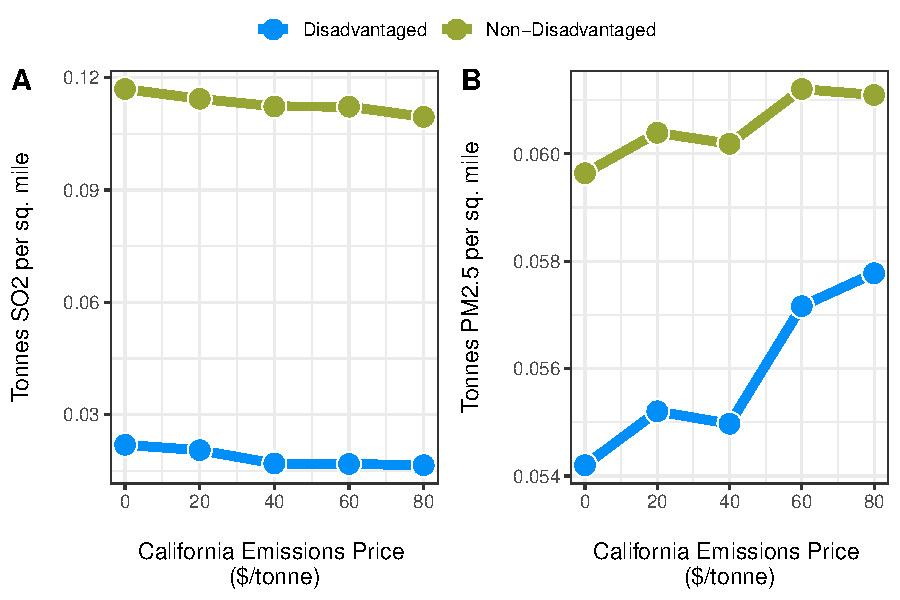
\includegraphics[width=\textwidth]{figures/chapter5_figures/ei_gap_so2_pm25.pdf}
    \fignote[1]{
        Figure shows the simulated average concentration of SO$_2$ and PM2.5 for DACs and non-DACs across five different carbon prices for Census tracts in the Western Interconnection. The distance between the two series is the EI Gap.
    }
\end{figure}


% \subsection{Diagnostics}





